\documentclass[11pt]{article}
\usepackage[a4paper, hmargin={2.8cm, 2.8cm}, vmargin={2.5cm, 2.5cm}]{geometry}
\usepackage{eso-pic} % \AddToShipoutPicture
\usepackage{graphicx} % \includegraPhics
\usepackage{placeins}
\usepackage{amsmath} % flere matematikkommandoer
\usepackage[utf8]{inputenc} % æøå
\usepackage[T1]{fontenc} % mere æøå
\usepackage{verbatim} % så man kan skrive ren tekst
\usepackage[all]{xy} % den sidste (avancerede) formel i dokumentet
\usepackage{amssymb}
\usepackage{listings}
\usepackage{hyperref}
\usepackage{multicol}
\usepackage{color}
\usepackage{url}
\usepackage{tcolorbox}
\usepackage{enumerate}
\usepackage{caption}
\usepackage{subcaption}
\usepackage{float}
\usepackage{glossaries}

\newacronym{POS}{POS}{Parts-of-Speech}
\newacronym{ISG}{ISG}{Integrated Syntactic Graph}
\newacronym{UBM}{UBM}{Universal Background Model}
\newacronym{AGS}{AGS}{Average Group Similarity}

\author{
    \Large{August Vinkel Soerensen \& Magnus Stavngaard} \\
    \texttt{august.vinkel@gmail.com \& magnus@stavngaard.dk} \\
}

\title{
    \vspace{3cm}
    \Huge{Authorship Verification} \\
    \Large{Project Outside Course Scope}
}

\usepackage{fancyhdr}
\pagestyle{fancy}

\lhead{University of Copenhagen}
\rhead{August Vinkel Soerensen \& Magnus Stavngaard}
%\cfoot{}
%\rfoot{\thepage}

\begin{document}

    \AddToShipoutPicture*{\put(0,0){\includegraphics*[viewport=0 0 700 600]{include/ku-farve}}}
    \AddToShipoutPicture*{\put(0,602){\includegraphics*[viewport=0 600 700 1600]{include/ku-farve}}}
    \AddToShipoutPicture*{\put(0,0){\includegraphics*{include/ku-en}}}
    \clearpage\maketitle
    \thispagestyle{empty}
    \newpage

    \section{Sumary}


    \newpage
    \tableofcontents
    \newpage

    \section{Introduction}
Authorship verification is the process of verifying the authorship of a text.
You are given a set of texts known to be written by the author and an unknown
text that has to be classified as either written by the author or someone else.
The normal approach to the problem is to use stylometry to extract features from
the text and then some form of machine learning or statistical method to analyse
the data \cite{stamatos2009}. A lot of different text features has been proposed
as describing an authors writing style. That includes but is not limited to
character frequencies, word frequencies, vocabulary size, sentence length,
punctuation usage, character n-grams, word n-grams and \gls{POS} tagging n-grams
\cite{stamatos2009}.

Authorship verification has been used for plagiarism control in danish secondary
schools \cite{hansen2014} and also has uses in civil law, criminal law and
computer forensics \cite{stamatos2009}.

In this article we explore state of the art methods for authorship verification.
We extract several different types of features including word frequencies, word
n-grams and pos-tagging n-grams. We implement several different algorithms to
work on the features. We start by implementing a baseline method which is a
distance based approach where an unknown text is considered to be written by
the closest author. We then use the baseline method to compare to our other
results. We use data from two sources \cite{pan:2015} and \cite{pan:2013} which
are two instances of a yearly competition in digital text forensics. Since we
use PAN data we also compare our results to the results obtained by others in
the competition.

% TODO: Continue.
%The PAN2013 and PAN2015 datasets are very different. The PAN2013 dataset
%contains many texts from a few authors while the PAN2015 texts contains a single
%text from many authors.


    \section{Related Work}


    \section{Feature Extraction}
%for example-
%Letter frequencies, N-gram frequencies, Function word usage, Vocabulary richness,
%Lexical richness, Distribution of syllables per word, Word frequencies, Hapax
%legomena, Hapax dislegomena, Word length distribution, Word collocations, Sentence
%length, Preferred word positions, Prepositional phrase structure, Distribution
%parts of speech, Phrasal composition grammar etc. [1][2][3][4][8][9]. The fact is that
%there is no such consensus on which stylometric features are applied to achieve the
%best results for authorship identification.
%
% Total Punctuation Count: This feature counts the number of total punctuation
%symbols used in a text, normalized by the word count in that text.
%
% Specific Punctuation Ratio: This is the ratio of the total number of specific
%punctuation symbols like comma (,), semicolon (;), question-mark (?), exclamation-mark
%(!), stop (.), slash (/), dash (-), colon (:) etc. to the total punctuation
%count.
%
% Long-sentence/ Short-sentence Ratio: Ratio of the long (length>12) or
%short (length<6) sentences to the total number of sentences is represented by
%this feature.
%
% Vocabulary Strength: We tried to capture the vocabulary strength of an author
%by calculating the ratio of the unique words used to the total number of
%words used in a text snippet.
%
% xPOS Frequency: In this feature, we try to capture the tendency of an author
%to use one or two particular types of POS that appear more frequently than
%the others, if there is any. So, we calculate the frequencies of each POS tag
%from texts and compare the known and unknown texts based on that.
%
% Starting POS Frequency: We try to list the POS tags that the author uses in
%the beginning of sentences according to their frequency and then compare
%them among the known and unknown documents to find a lexical pattern.
%For example, a particular author might have the tendency to start sentences
%with auxiliary verbs (example) or prepositions (in, for) unknowingly for a
%considerable number of sentences in the corpus. The feature also indicates
%the writing style of the author.
%In the above example, both known
%
% FROM maitra2015




% From Castro:2015
%1. Character
%(a) Tri-grams of characters (F1)
%(b) Quad-grams of characters (F2)
%(c) Word prefixes of size 2 (F3)
%(d) Word suffixes of size 2 (F4)
%2. Words
%(a) Uni-grams of words (F5)
%(b) Tri-grams of words (F6)
%3. Lemma and Part of Speech
%(a) Uni-grams of lemmas (F7)
%(b) Uni-grams of Part of Speech (F8)
%(c) Tri-grams of lemmas (F9)
%(d) Tri-grams of Part of Speech (F10)


    \section{Machine Learning}


    % TODO: Report both TPR and TNR for all methods.
\section{Results} \label{sec:results}
As described earlier the PAN 2013 results are ranked using the F1 measure. The
measure is defined using \textit{precision} and \textit{recall} which in PAN
2013 is defined as,

\begin{align}
    precision &=  \frac{correct\_answers}{answers} \\[1em]
    recall &= \frac{correct\_answers}{problems}
\end{align}

Since we answer all problems $problems$ and $answers$ are the same in our case
and therefore we get that the F1 measure is the same as an accuracy,

\begin{equation}
    F1 = 2 \frac{precision \cdot recall}{precision + recall}
        = 2 \frac{accuracy^2}{2accuracy}
        = \frac{2accuracy^2}{2accuracy}
        = \frac{accuracy^2}{accuracy}
        = accuracy.
\end{equation}

Similarly as described earlier the PAN 2015 results are ranked using the product
of \gls{AUROC} and c@1. The \gls{AUROC} is a measure of discrimination. That
is, it measures the ability of a solution to distinguish between texts written
by the same author and texts written by another author. An \gls{AUROC} score is
generally considered excellent when between 0.9 and 1, good when between 0.8
and 0.9, fair when between 0.7 and 0.8, poor when between 0.6 and 0.7 and a
failure when between 0.5 and 0.6. The c@1 measure is chosen since it measures
performance in the binary case. The c@1 measure does not use probabilities but
classifies everything above 0.5 as a yes everything below as a no and a 0.5 as a
don't know. Like F1 in PAN 2015 the c@1 also corresponds to an accuracy in our
case since we answer all questions. The definition of c@1 is,

\begin{equation}
    c@1 = \frac{1}{n} \left(n_c + \frac{n_u \cdot n_c}{n}\right)
\end{equation}

where $n$ is the number of problems, $n_c$ is the number of correct answers and
$n_u$ is the number of unanswered problems. So when $n_u$ is 0 we have,

\begin{equation}
    c@1 = \frac{1}{n} \left(n_c + \frac{n_u \cdot n_c}{n}\right)
        = \frac{1}{n} \left(n_c + \frac{0 \cdot n_c}{n}\right)
        = \frac{1}{n} n_c
        = accuracy.
\end{equation}

In this section we will describe how we have tested our solutions on the test
datasets and give the results of those tests. When we are testing on the PAN
2013 dataset we will report an accuracy as that is the only performance measure.
When we are testing on the PAN 2015 dataset we will report both the \gls{AUROC}
and the accuracy since both are used to measure performance.

\subsection{Delta Method} \label{subsec:results:delta_method}
The Delta method was tested by creating the same features for both the training
dataset and the test datasets. We then computed the mean and standard variance
of the training set and used that to normalize both the training and test
dataset. For each text in the test dataset we then drew differing numbers of
opposing texts from the training dataset. Those opposing texts were used as
the opposition in the Delta Method. The number of opposing authors we used
were the ones we found in the training section and were 4 for PAN 2013 and 1
for PAN 2015. The results for running the delta method on the two test sets
included in PAN 2013 and one dataset included in PAN 2015 is shown in Table
\ref{tab:delta_method_final_results}. The \gls{AUROC} curve for the Delta Method
is shown in Figure \ref{fig:delta_method_roc}. It is created by computing the
\gls{TPR} and \gls{FPR} for the differing number of opposing authors.

\begin{table}
    \centering
    \begin{tabular}{c|ccc}
        & \textbf{PAN 2013 Dataset 1} & \textbf{PAN 2013 Dataset 2} & \textbf{PAN 2015 Dataset}\\
        \hline
        \textbf{Accuracy}  & 0.63191 & 0.61314 & 0.55480 \\
        \textbf{\gls{TPR}} & 0.51900 & 0.52492 & 0.50820 \\
        \textbf{\gls{TNR}} & 0.72408 & 0.70000 & 0.60140
    \end{tabular}
    \caption{Result of running the delta method on two test sets included in PAN
    2013 and single test set included in PAN 2015 with 4 opposing authors for
    the PAN 2013 set and 1 opposing author for PAN 2015.}
    \label{tab:delta_method_final_results}
\end{table}

The \gls{AUROC} for the delta method on the 2015 data was 0.56378. Resulting
in a final score of $0.55480 \cdot 0.56550 = 0.31373$ for the PAN 2015 set.

\begin{figure}
    \centering
    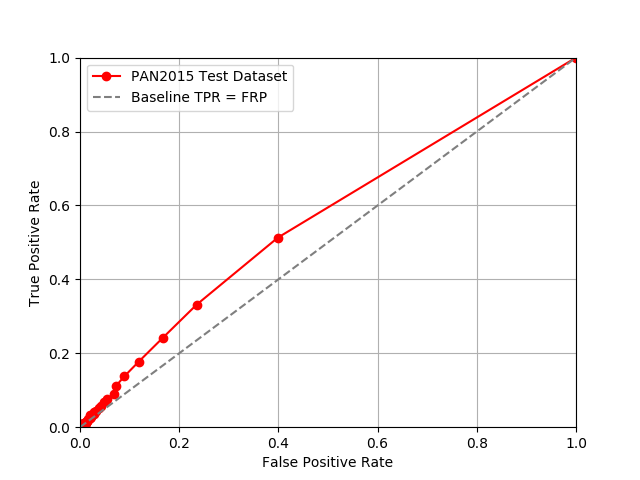
\includegraphics[width=.7\textwidth]{./pictures/delta_method_roc.png}
    \caption{The ROC curve of the delta method with number of opposing authors
    varying from 0 to 100 using the test dataset for PAN 2015.}
    \label{fig:delta_method_roc}
\end{figure}

\subsection{Generalising Random Forest} \label{subsec:results:generalising_random_forest}
In order to test the \gls{UBM} approach proposed by \cite{pacheco2015}, we start
by computing our feature set and generating our \gls{UBM} as described in
Section \ref{subsec:method:generalising_random_forest}.

The feature set and \gls{UBM}, are then encoded according to Equation
\eqref{eq:rf-encode}, and are used to train a random forest with parameters
matching the ones used in experiments. That is all parameters being set to their
default except \texttt{n\_estimators} that is set to 1000. At this point we
encode the feature set created from the test data, against the \gls{UBM}, which
is then fed to our trained random forest to get the predictions. This resulted
in an accuracy of 0.60400, \gls{TPR} of 0.63200 and \gls{TNR} of 0.57600 on the
pan 2015 dataset. On the other hand, we also chose to train our model using the
alternate subtraction encoding, which doesn't make use of the \gls{UBM}. The
subtraction encoding under-performed relative to the \gls{UBM} approach, with an
accuracy of 0.58400 a \gls{TPR} of 0.66800 and a \gls{TNR} of 0.50000.

We have generated the \gls{ROC} curve for both random forest tests. The area
under the curve was 0.63868 for the \gls{UBM} method and 0.56821 for the Minus
method. The curves is shown in Figure \ref{fig:forest_roc}. This means that the
Final Score, of the methods are the following:

\begin{align}
    \text{Final Score \gls{UBM}} &= c@1 \cdot AUROC = 0.604 \cdot 0.63868 = 0.3858  \\
    \text{Final Score Minus} &= c@1 \cdot AUROC = 0.584 \cdot 0.56821 = 0.3318
\end{align}

The curve was generated by computing the probability for each problem of the
answer being "same author". Then different thresholds for when a answer is
considered "same author" can be tried and the \gls{TPR} and \gls{FPR} can be
computed for all thresholds. In our case we tried the thresholds $\{0.0, 0.01,
\dots, 1.0\}$.

\begin{figure}
    \centering
    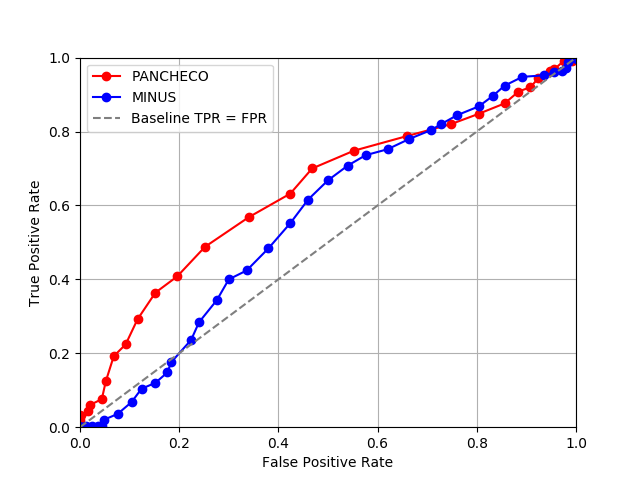
\includegraphics[width=.7\textwidth]{./pictures/forest_roc.png}
    \caption{The ROC curve of the two Generalising Random Forest
    approaches.}
    \label{fig:forest_roc}
\end{figure}

\subsection{Extended Delta} \label{subsec:results:extended_delta}
The Extended Delta Method is tested by generating features according to the best
configurations found in the training phase. Then the same procedure used to
test the regular delta method is employed. The best configuration for the PAN
2013 data were the 100 most frequent 2-, 3-, and 4-char-grams and the 300 most
frequent words for 5 opposing authors. The best configuration for the PAN 2015
data were the 20 most frequent 1-, 2-, and 3-special-char-grams for 2 opposing
authors. The accuracies, \gls{TPR}s and \gls{TNR}s obtained on all test datasets
are shown in Table \ref{tab:extended_delta_method_final_results}. The \gls{ROC}
curve is shown in Figure \ref{fig:extended_delta_method_roc} and the \gls{AUROC}
was 0.65188.

\begin{table}
    \centering
    \begin{tabular}{c|ccc}
        & \textbf{PAN 2013 Dataset 1} & \textbf{PAN 2013 Dataset 2} & \textbf{PAN 2015 Dataset} \\
        \hline
        \textbf{Accuracy}  & 0.72528 & 0.67291 & 0.61949 \\
        \textbf{\gls{TPR}} & 0.66750 & 0.75761 & 0.49760 \\
        \textbf{\gls{TNR}} & 0.77244 & 0.58953 & 0.74140
    \end{tabular}
    \caption{Result of running the extended delta method on two test sets
    included in PAN 2013 and single test set included in PAN 2015 with the best
    configurations found in the training phase.}
    \label{tab:extended_delta_method_final_results}
\end{table}

\begin{figure}
    \centering
    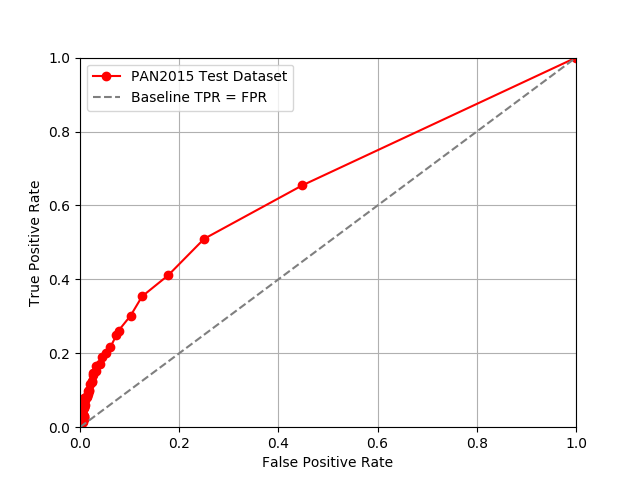
\includegraphics[width=.7\textwidth]{./pictures/extended_delta_method_roc.png}
    \caption{The ROC curve of the Extended Delta Method with number of opposing
    authors varying from 0 to 100 using the test dataset for for PAN 2015.}
    \label{fig:extended_delta_method_roc}
\end{figure}

\subsection{Author Specific SVM} \label{subsec:results:author_specific_svm}
The Author Specific SVM is tested by generating features for the training and
test datasets for the PAN 2013 texts. For each different author in the test
dataset we extract features for all their known texts and their single unknown
text. We then draw random texts from the training dataset which will serve as
opponents to the texts written by the author. Then we train an SVM using the
texts known to be written by the author and the texts from the training dataset
and predict the unknown text using that SVM.

The best configuration on the training set were configuration B using the
frequencies of the 300 most frequent words. The results on the two test datasets
are shown in Table \ref{table:svm_results}.

\begin{table}
    \centering
    \begin{tabular}{c|cc}
        & \textbf{Test Dataset 1} & \textbf{Test Dataset 2} \\
        \hline
        \textbf{Accuracy}  & 0.77650 & 0.78066 \\
        \textbf{\gls{TPR}} & 0.71444 & 0.70785 \\
        \textbf{\gls{TNR}} & 0.82727 & 0.84437
    \end{tabular}
    \caption{Results of the Author Specific SVM on the two test datasets for PAN
    2013.}
    \label{table:svm_results}
\end{table}


    \section{Conclusion} \label{sec:conclusion} 

We presented a collection of machine learning and distance based approaches
to the PAN 2013, and PAN 2015 tasks. We set out to beat the baseline a baseline
method, which in our case was the Delta Method, using a subset of algorithmic
approaches used on the two PAN tasks.

While we did succeed in doing so, the results produced for the two different
tasks were vastly different. This stems from the different nature of each of
the PAN tasks. While they both serve to verify if a person is indeed the author
of a specific text, the format of the data in the two tasks, results in vastly
different methods having to be used. As mentioned earlier, the PAN 2015 data-set
contains very little data. It does have a lot of data entries in the form of
authors, but each author only has 1 known text, and that texts' length has an
average word count of 460. After implementing several algorithm, it became
obvious that this data was more suited for a generalizing approach, due to the
high author count. This however contradicted the more appropriate approaches
for the 2013 set. With its numerous text per author, and its 1038 average word
count, the PAN 2013 set was more suited for approaches which made use of the
larger quantities of data the set provided. This different is showcased by the
performance of the Generalizing random forest and the SVM. The encoding used
for the random forest was used to get around the data lack of data in the 2015
set, by creating a generalizing model instead. Thus depending on the amount of
authors, instead of the amount of data. This resulted in the performance on the
2013 set, to be far inferior compared to the 2015 set. On the other hand, the
SVM bases itself on the large amount of data entries per author. If one was to
use that on the 2015 set, one would have to split the singular text for each
author up, to then get more data, thus further diluting the already sparse data
set, ending up with poor results.

One thing worth noting however, was that the importance of stop word was way 
above expectation. Looking at the feature importance graphs for the 
generalizing random forest, we can see that stop words in has
a great impact the classification. Not only that by special characters,
does as well, most likely due to the information about sentence composition it
conveys.



\begin{itemize}
    \item Answer the problem presented in the abstract
    \item Specific stop word features might have been good for performance.
    \item Generating opposing set from external source might have lead to better
        performance.
    \item The problem is much easier when more data is available.
    \item The problem changes depending on the data
    \item Were able to beat all baseline methods.
    \item Performed very well on PAN 2013 but not so well on PAN 2015.
\end{itemize}


    \section{Discussion} \label{sec:discussion}

\subsection{Comparison to baseline approach}
Our baseline approach was the Delta Method described in Section
\ref{subsec:method:delta_method}. One of the goals of this report was finding
and implementing methods for authorship verification that could beat our
baseline method. An overview of the different methods final results can be seen
in Table \ref{tab:all_final_results}. It can be seen that we were able to beat
the baseline method both on the PAN 2013 dataset and the PAN 2015 dataset.

% TODO: Maybe elaborate on what it means that we beat the baseline methods.

\begin{table}
    \centering
    \begin{tabular}{|c|c|c|c|}
    \hline
    \textbf{Method}             & \textbf{P2013.1 F1 Score} & \textbf{P2013.2 F1 Score} & \textbf{P2015 Final Score} \\ \hline
    Delta (BASELINE)            & 0.64438                      & 0.63291                      & 0.3188                        \\ \hline
    Random Forest (\gls{UBM}) & -                            & -                            & 0.3858                        \\ \hline
    Random Forest (Minus)       & -                            & -                            & 0.3318                        \\ \hline
    Extended Delta              & 0.73213                      & 0.67173                      & 0.4053                        \\ \hline
    SVM                         & 0.77650                      & 0.78066                      & -                             \\ \hline
    \end{tabular}
    \caption{Final results for all our implemented algorithms for authorship
    verification on the datasets that apply to the method.}
    \label{tab:all_final_results}
\end{table}

\subsection{Comparison to other PAN results}

Throughout the making of this paper, several oddities occurred, which needs
addressing in order to better understand the behavior of our implemented
verification models. In in the real world, authorship-verification problems
like this are especially relevant for companies like MaCom, who operates a
website, used for submission of high-school students assignments throughout
Denmark. While both the PAN 2013, and PAN 2015 tasks aim is to implement
authorship-verification, they both represent extremes in that very area. PAN
2013, lends itself very well to author specific methods, as it contains a lot of
text for each author, but a small amount of authors, and PAN 2015 lends itself
more to the generalized approach due to the small amount of text per author. As
such, relating our method to the real world example of MaCom might give some
perspective as well. The data MaCom has, closely resembles the data from the PAN
2013 task. However, with a lot more authors and no unknown text.

Starting off with the Generalized Random Forest
\ref{subsubsec:method:generalizing_random_forest}. This method was off to a bad
start, as the paper it was based on \cite{pacheco2015} only got 6'th place in
the PAN 2015 authorship verification task, and our implementation of that same
method only ranked 9'th. \ref{subsec: Pan2015Res} The main focus of this method
however, was the way it attempted to circumvent the lack of data, associated
with each specific author, by instead learning on the know-text dataset in
its entirety. This approach, actually worked as seen in the test results. By
learning based on a \gls{UBM}, we were able to improve the results compared to
learning on the author-specific feature difference. The lack of text associated
with each author also left quite an impact in terms of what features were
relevant. After training our random forest model, it became apparent that there
was no case where word N-grams performed well, in terms of the classification.
The suspected reason for this, might be that very lack of text. The texts being
limited to about 150 words, means that there are only that many word N-grams in
the text, which limit the variety of word N-grams. However, the word-N-grams
extracted from the brown corpus, varies a lot, and as such only a few of the
word-N-grams extracted from the brown corpus are in the actual text, this only
becomes more evident as N increases due to the limited size of the texts. As
such, while the feature might very will have a high impact in some cases, we
suspect the impact will be averaged out over all the trees in the random forest.

If this \gls{UBM} method was to be applied to the MaCom data set, time
complexity would also have to analyzed in order to determine the viability of
the Generalized RF method. By only considering $\log(N)$ features in our case,
where N is the total number of features, we are able to handle large amount of
data. The time complexity of the method can be broken down into two parts. The
creating of a tree, and number of features considered. The time complexity of a
single decision tree, is $O(n \log{n})$, where n is the total number of leafs on
the tree. In our case, each tree considers $\log{N}$ features. This gives us a
final time complexity of $O(\log{N} \cdot n \log{n})$.\cite{RFTime}

While the method didn't provide any impressive results, the generalized approach
might very well be useful in the future, in case one comes across another data
sparse set. An improvement that could be done however, was to increase the
number of features fed to the random forest. Not only quantity, but also
different types of features than the ones used in this paper. This would
work since Random Forest by its' very nature selects the best features for
classification, we can at the cost of some run time, train on a much larger
feature-set and we suspect better results some might be produced.

\begin{itemize}
    \item Why did the delta method perform so much better on the training data?
    \item Comparison of our test results to the best ones in PAN 2013 and PAN
        2015.
    \item How does different methods scale to huge amounts of data?
    \item Discuss potential usage in future project based on TPR and TNR.
    \item What improvements could be made to any of the method used. RF Done
    \item Why did SVM's perform so well (https://link.springer.com/article/10.1023/A:1023824908771).
        \begin{itemize}
            \item SVM's can handle many thousands of features.
        \end{itemize}
    \item Manhattan performs better than euclidean in extended delta.
\end{itemize}


    \section{Future Work} \label{sec:future_work}

Two of the algorithm we have implemented has only been applied to one of the
two datasets we have worked with. In particular the Random Forest approach has
only been applied to the PAN 2015 data and the \gls{SVM} approach has only been
applied to the PAN 2013 data. The main reason for that, is that the Random
Forest approach requires a single known text per author and the \gls{SVM}
approach require multiple known texts per author. It would be interesting to
apply the algorithms to the opposite datasets and look at their performance
there. We can transform the dataset with only a single known text to a dataset
with multiple by splitting the known text into a collection of known texts.
Similarly we can transform the dataset with multiple known texts to a dataset
with a single known text by concatenating the known texts. By making those two
transformations we could have run all methods on all data and found results for
all of them.

We would also like to apply our different implemented methods to larger
datasets. We have found in this assignment that having more text available per
author improves the performance of our methods. All our implemented methods
performed better on the PAN 2013 dataset than on the PAN 2015 dataset. For
example there is a Danish company, MaCom, that produce software for turning in
and managing school assignments. MaCom has a large database containing several
texts for each student and they have an interest in authorship verification.
They specifically want to verify that assignments uploaded by students match
their previous assignments and are not written by someone else. MaCom's main
requirement is a method that has a high \gls{TPR}. The reason is that they
don't want to falsely accuse anyone of not having written their own assignment,
while it doesn't matter as much if they miss some assignment that is written by
someone else. When the \gls{TPR} is high it means that there is few \gls{FN}s
and many \gls{TP}s. \gls{FN}s are as described earlier when we say a text is
written by a different author while it is actually written by the same.

Since MaCom has much data available per student their case most closely match
that of the PAN 2013 dataset. The method we implemented with the best \gls{TPR}
on the PAN 2013 dataset was our Extended Delta Method approach. So it would be
interesting to apply that approach to MaCom's dataset. The \gls{SVM} approach
also had a very promising \gls{TPR} on the training dataset so it would also be
interesting to try that.


    \nocite{*} % TODO: Consider if this should be removed.
    \bibliographystyle{apalike}
    \bibliography{literature}

\end{document}
